\documentclass[letterpaper,10pt]{article}

\usepackage{enumitem}
\usepackage{titling}
\usepackage{listings,listings-rust}
\usepackage{url}
\usepackage{soul}
\usepackage{hyperref}
\usepackage{setspace}
\usepackage{subfig}
\usepackage{sectsty}
\usepackage{pdfpages}
\usepackage{colortbl}
\usepackage{multirow}
\usepackage{multicol}
\usepackage{relsize}
\usepackage{amsmath}
\usepackage{wasysym}
\usepackage{fancyvrb}
\usepackage[yyyymmdd]{datetime}
\usepackage{amsmath,amssymb,amsthm,graphicx,xspace}
\usepackage[titlenotnumbered,noend,noline]{algorithm2e}
\usepackage[compact]{titlesec}
\usepackage{XCharter}
\usepackage[T1]{fontenc}
\usepackage[scaled]{beramono}
\usepackage[normalem]{ulem}
\usepackage{booktabs}
\usepackage{tikz}
\usetikzlibrary{arrows.meta,automata,shapes,trees,matrix,chains,scopes,positioning,calc,decorations.pathreplacing}
\tikzstyle{block} = [rectangle, draw, fill=blue!20, 
    text width=2.5em, text centered, rounded corners, minimum height=2em]
\tikzstyle{bw} = [rectangle, draw, fill=blue!20, 
    text width=4em, text centered, rounded corners, minimum height=2em]

\definecolor{namerow}{cmyk}{.40,.40,.40,.40}
\definecolor{namecol}{cmyk}{.40,.40,.40,.40}
\renewcommand{\dateseparator}{-}

\let\LaTeXtitle\title
\renewcommand{\title}[1]{\LaTeXtitle{\textsf{#1}}}

\lstset{basicstyle=\footnotesize\ttfamily,breaklines=true}

\newcommand{\CPP}{C\nolinebreak\hspace{-.05em}\raisebox{.4ex}{\tiny\bf +}\nolinebreak\hspace{-.10em}\raisebox{.4ex}{\tiny\bf +}}
\def\CPP{{C\nolinebreak[4]\hspace{-.05em}\raisebox{.4ex}{\tiny\bf ++}}}

\newcommand{\handout}[5]{
  \noindent
  \begin{center}
  \framebox{
    \vbox{
      \hbox to 5.78in { {\bf ECE459: Programming for Performance } \hfill #2 }
      \vspace{4mm}
      \hbox to 5.78in { {\Large \hfill #4  \hfill} }
      \vspace{2mm}
      \hbox to 5.78in { {\em #3 \hfill \today} }
    }
  }
  \end{center}
  \vspace*{4mm}
}

\newcommand{\lecture}[3]{\handout{#1}{#2}{#3}{Lecture#1}}
\newcommand{\tuple}[1]{\ensuremath{\left\langle #1 \right\rangle}\xspace}

\addtolength{\oddsidemargin}{-1.000in}
\addtolength{\evensidemargin}{-0.500in}
\addtolength{\textwidth}{2.0in}
\addtolength{\topmargin}{-1.000in}
\addtolength{\textheight}{1.75in}
\addtolength{\parskip}{\baselineskip}
\setlength{\parindent}{0in}
\renewcommand{\baselinestretch}{1.5}
\newcommand{\term}{Winter 2020}

\singlespace


\begin{document}

\lecture{4 --- Cache Coherency}{\term}{Patrick Lam \& Jeff Zarnett}

\section*{Cache Coherency}

\begin{center}
    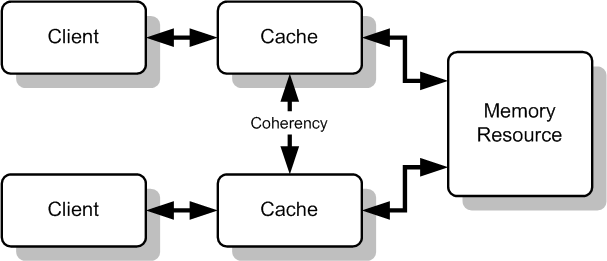
\includegraphics[width=0.5\textwidth]{images/coherency}

\hfill ---Wikipedia
\end{center}

Today we'll look at what support the architecture provides for memory ordering, in
particular in the form of cache coherence. Since this isn't an
architecture course, we'll look at this material more from the point
of view of a user, not an implementer.

The problem is, of course, that each CPU likely its own cache. If it does then these data may be out of sync -- the value that CPU 1 has for a particular piece of data might be different from the value that CPU 4 has. The simplest method, and a horrible solution, would be the ability to declare some read/write variables as being non-cacheable (is that a word? Uncacheable?...). The compiler and OS and such will require the data to be read from main memory, always. This will obviously result in lower cache hit ratios, increased bus traffic, and terrible, terrible performance. Let's avoid that. What we want instead is \textit{coherency}.

Cache coherency means that:
  \begin{itemize}
    \item the values in all caches are consistent; and
    \item to some extent, the system behaves as if all CPUs are using shared memory.
  \end{itemize}
  
In modern CPUs with three or four levels of cache, we frequently find that the level 3 cache isn't much faster than going to main memory. But this level is where the cache coherency communication can take place. This can be by making the cache shared between the different CPUs. And the L4 cache is frequently used for sharing data with the integrated graphics hardware on CPUs that have this feature. But for the most part we will imagine that caches are not shared, and we have to figure out how to get coherency between them. This is the case with a L1/L2 cache in a typical modern CPU as they are unique to the given core (i.e., not shared).
  
\paragraph{Cache Coherence Example.} We will use this example to illustrate
different cache coherence algorithms and how they handle the same situation.

Initially in main memory: {\tt x = 7}.

  \begin{enumerate}
    \item {\tt CPU1} reads x, puts the value in its cache.
    \item {\tt CPU3} reads x, puts the value in its cache.
    \item {\tt CPU3} modifies {\tt x := 42}
    \item {\tt CPU1} reads x \ldots ~from its cache?
    \item {\tt CPU2} reads x. Which value does it get?
  \end{enumerate}

Unless we do something, {\tt CPU1} is going to read invalid data.
  
Outside of a computing context, imagine you and several co-workers have some shared information, such as a meeting (in a specific room) in a shared online calendar (the one for the room). You (or anyone else) could make changes to this event. As mind-reading does not work, there are two ways that another invitee can know that something has changed: (1) they can check to see if anything has changed, or (2) they can be notified that a change has occurred. 

The notification may contain the updated information in its entirety, such as ``Event title changed to 'Discuss User Permissions and Roles''', or it may just tell you ``something has changed; please check''. In transportation, you can experience both... in the same day. I [JZ] was flying to Frankfurt and going to catch a train. Air Canada sent me an e-mail that said ``Departure time revised to 22:00'' (20 minute delay); when I landed the Deutsche Bahn (German railways) sent me an e-mail that said ``Something on your trip has changed; please check and see what it is in the app''... it was my train being cancelled. I don't know why they couldn't have e-mailed me that in the first place! It's not like I was any less annoyed by finding out after taking a second step of opening an app.

Regardless of which method is chosen, we have to pick one. We can't pick none of those and expect to get the right answers.


\paragraph{Snoopy Caches.} The simplest way to ``do something''
is to use Snoopy caches~\cite{snoopycache}. No, not this kind of Snoopy (sadly):

\begin{center}
	
\includegraphics[width=0.3\textwidth]{images/peanuts-snoopy1.jpg}
\end{center}

It's called Snoopy because the caches are, in a way, spying on each other: they are observing what the other ones are doing. This way, they are kept up to date on what's happening and they know whether they need to do anything. They do not rely on being notified explicitly. This is a bit different from the transportation analogy, of course, but workable in a computer with a shared bus.

This is a distributed approach; no centralized state is maintained. Each cache with a copy of data from a block of main memory knows whether it is shared or not. All the CPUs are connected to a shared bus, and each CPU has its own cache controller. Whenever a CPU issues a memory write, the other CPUs are watching (colloquially, ``snooping around'') to observe if that memory location is in their cache. If so, the CPU will need to take action.

What does action mean? In the flight plus train example, both kinds of action occurred. The Air Canada action was \textit{update} -- the information about the flight departure time was changed from 21:40 to 22:00 and at the time of becoming aware of the change, I got the new value immediately. The Deutsche Bahn action was \textit{invalidate} -- the information about the train was changed, but I didn't know what had changed. All that I really knew is that the old information I had was out of date. When I needed that information again, I had to go get it myself from the source (their app). Either action (noting down the new, or knowing that what I have is out of date) is adequate for ensuring that I have the most up to date information. You may have a preference on which one you think is better, but unfortunately this is not your decision, neither as a user of the hardware of the computer nor as  a person who wants to travel by plane or train.

\subsection*{Write-Through Caches}
Let's put that into practice using write-through caches, the simplest type of
cache coherence.
  \begin{itemize}
    \item All cache writes are done to main memory.
    \item All cache writes also appear on the bus.
    \item If another CPU snoops and sees it has the same location in
      its cache, it will either invalidate or update the
      data.
  \end{itemize}
  
Invalidation is the most common protocol. It means the data in the cache of other CPUs is not updated, it's just noted as being out of date (invalid).  Normally, when you write to an invalidated location, you bypass the cache and go directly to memory (aka {\bf write no-allocate}). This kind of thing happens if you're just doing \texttt{x = 42;} -- it doesn't matter what value of \texttt{x} was there before; you're just overwriting it.

If we want to do a read and there's a miss, we can ask around the other caches to see who has the most recent cached version. This is a bit like going into a room and yelling ``Does anybody have block...?'', in some sort of multicast version of the card game ``Go Fish''. Regardless, the most recent value appears in memory, always, so if nobody else has it in cache (or they don't feel like sharing) you can get it from there.

There are also write broadcast protocols, in which case all versions in all caches get updated when there is a write to a shared block. But it uses lots of bandwidth and is not necessarily a good idea. It does, however prevent the costly cache miss that follows an invalidate. Sadly, as we are mere users and not hardware architects, we don't get to decide which is better; we just have to live with whichever one is on the hardware we get to use. Bummer.

\paragraph{Write-Through Protocol.}
The protocol for implementing such caches looks like this.
There are two possible states, {\bf valid} and {\bf invalid}, for each cached memory location.
Events are either from a processor ({\bf Pr}) or the {\bf Bus}. Actions will be either a \textbf{Rd} (read) or \textbf{Wr} (write).
We then implement the following state machine.

  \begin{center}
    \begin{tabular}{l|l|l|l}
      {\bf State} & {\bf Observed} & {\bf Generated} & {\bf Next State}\\ \hline
      Valid   & PrRd  &       & Valid\\
      Valid   & PrWr  & BusWr & Valid\\
      Valid   & BusWr &       & Invalid\\
      Invalid & PrWr  & BusWr & Valid\\
      Invalid & PrRd  & BusRd & Valid\\
    \end{tabular}
  \end{center}

\paragraph{Example.} For simplicity (this isn't an architecture course), assume all cache
      reads/writes are atomic. \footnote{If you're a hardware person, this line probably makes you cry. There's a whole lot that goes into making this work. There are potential write races, which have to be dealt with by contending for the bus and then completing the transaction, possibly restarting a command if necessary. If we have a split transaction bus it's really ugly, because we can have multiple interleaved misses. And down the rabbit hole we go.} Using the same example as before:

Initially in main memory: {\tt x = 7}.

  \begin{enumerate}
    \item {\tt CPU1} reads x, puts the value in its cache. {(valid)}
    \item {\tt CPU3} reads x, puts the value in its cache. {(valid)}
    \item {\tt CPU3} modifies {\tt x := 42}. {(write to memory)}
      \begin{itemize}
        \item {{\tt CPU1} snoops and marks data as invalid.}
      \end{itemize}
    \item {\tt CPU1} reads x, {from main memory. (valid)}
    \item {\tt CPU2} reads x, {from main memory. (valid)}
  \end{enumerate}

\subsection*{Write-Back Caches}
Let's try to improve performance. What if, in our example, {\tt CPU3} writes to {\tt x} 3 times in rapid succession? It's unpleasant to have to flush that to memory three times when we could do it only once. Let's try to delay the write to memory as long as possible. At minimum, we need support in hardware for a ``dirty'' bit, which indicates the our data has been changed but not yet been written to memory.

\paragraph{Write-Back Implementation.}
     The simplest type of write-back protocol (MSI) uses 3 states instead of 2:
      \begin{itemize}
        \item {\bf Modified}---only this cache has a valid copy; 
          main memory is {\bf out-of-date}.
        \item {\bf Shared}---location is unmodified, 
           up-to-date with main
          memory; 
          \quad may be present in other caches (also up-to-date).
        \item {\bf Invalid}---same as before.
      \end{itemize}
      
The initial state for a memory location, upon its first read, is ``shared''.
The implementation will only write the data to memory if another
processor requests it.
During write-back, a processor may read the data from the bus.

\paragraph{MSI Protocol.} Here, bus write-back (or flush) is {\bf BusWB}.
Exclusive read on the bus is {\bf BusRdX}.

\begin{center}
    \begin{tabular}{l|l|l|l}
      {\bf State} & {\bf Observed} & {\bf Generated} & {\bf Next State}\\ \hline
      Modified   & PrRd   &        & Modified\\
      Modified   & PrWr   &        & Modified\\
      Modified   & BusRd  & BusWB  & Shared\\
      Modified   & BusRdX & BusWB  & Invalid\\
      Shared     & PrRd   &        & Shared\\
      Shared     & BusRd  &        & Shared\\
      Shared     & BusRdX &        & Invalid\\
      Shared     & PrWr   & BusRdX & Modified\\
      Invalid    & PrRd   & BusRd  & Shared\\
      Invalid    & PrWr   & BusRdX & Modified\\
    \end{tabular}
\end{center}

\paragraph{MSI Example.} Using the same example as before:

Initially in main memory: {\tt x = 7}.

  \begin{enumerate}
    \item {\tt CPU1} reads x from memory. {(BusRd, shared)}
    \item {\tt CPU3} reads x from memory. {(BusRd, shared)}
    \item {\tt CPU3} modifies {\tt x = 42}:
      \begin{itemize}
        \item {Generates a BusRdX.}
        \item {{\tt CPU1} snoops and invalidates x.}
      \end{itemize}
    \item {\tt CPU1} reads x:
      \begin{itemize}
        \item {Generates a BusRd.}
        \item {{\tt CPU3} writes back the data and sets x to shared.}
        \item {{\tt CPU1} reads the new value from the bus as shared.}
      \end{itemize}
    \item {\tt CPU2} reads x from memory. {(BusRd, shared)}
  \end{enumerate}

\subsection*{An Extension to MSI: MESI}
    The most common protocol for cache coherence is MESI.
    This protocol adds yet another state:
      \begin{itemize}
        \item {\bf Modified}---only this cache has a valid copy; 
 main memory is {\bf out-of-date}.
        \item {\bf Exclusive}---only this cache has a valid copy; 
 main memory is {\bf up-to-date}.
        \item {\bf Shared}---same as before.
        \item {\bf Invalid}---same as before.
      \end{itemize}

    MESI allows a processor to modify data exclusive to it, without
    having to communicate with the bus.  MESI is safe. The key is that
    if memory is in the E state, no other processor has the data. The transition from E to M does not have to be reported over the bus, which potentially saves some work and reduces bus usage. 

\subsection*{MSEIF: Even More States!}

    MESIF (used in latest i7 processors):
      \begin{itemize}
        \item {\bf Forward}---basically a shared state; but, current
          cache is the only one that will respond to a request to
          transfer the data.
      \end{itemize}

    Hence: a processor requesting data that is already shared or exclusive will
      only get one response transferring the data. Under a more simple MESI scheme you could get multiple caches trying to answer, with leads to bus arbitration or contention. The existence of a F state permits more efficient usage of the bus.
      
      
\subsection*{False Sharing}
False sharing is something that happens when our program has two unrelated data elements that are mapped to the same cache line/location. Let's consider an example from~\cite{falsesharing}:

\begin{lstlisting}[language=C]
char a[10];
char b[10];
\end{lstlisting}
These don't overlap but are almost certainly allocated next to each other in memory. If a thread is writing to \texttt{a} and they share a cache line, then \texttt{b} will be invalidated and the CPU working on \texttt{b} will be forced to fetch the newest value from memory. This can be avoided by seeing to it that there is some separation between these two arrays.

One way would be to heap allocate both arrays. You can find where things are located, if you are curious, by printing the pointer (or the address of a regular variable). Usually if you do this you will find that they are not both located at the same location. But you are provided no guarantee of that. So the other alternative is to make both arrays bigger than they need to be such that we're sure they don't overlap.

Consider the graph below that shows what happens in a sample program reading and writing these two arrays, as you increase the size of arrays \texttt{a} and \texttt{b} (noting that byte separation of 11 means they are adjacent; anything less than that and they overlap). This does waste space, but is it worth it?

\begin{center}
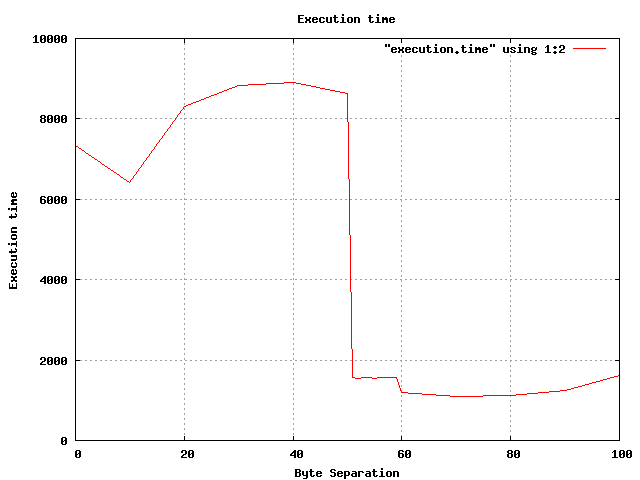
\includegraphics[width=0.6\textwidth]{images/falsesharing.png}\\
Execution time graph showing 5x speedup by ``wasting'' some space~\cite{falsesharing}.
\end{center}

At separation size 51 there is a huge drop in execution time because now we are certainly putting the two arrays in two locations that do not have the false sharing problem. Is wasting a little space worth it? Yes!

P.S. putting these arrays in a struct and padding the struct can also help with enabling future updates to the struct.

\subsection*{Volatile}

\begin{quote}
``Well, I read that {\tt volatile} variables aren't stored in registers,
    so then am I okay?''
\end{quote}

Again, sadly, no. Recall that {\tt volatile} in C was only designed to~\cite{pr:volatile}:
      \begin{itemize}
        \item Allow access to memory mapped devices.
        \item Allow uses of variables between {\tt setjmp} and {\tt longjmp}.
        \item Allow uses of {\tt sig\_atomic\_t} variables in signal handlers.
      \end{itemize}

All of these things apply to single-threaded situations or cases where the compiler has re-ordered some steps. Remember, things can also be reordered by the compiler, and {\tt
  volatile} doesn't prevent reordering. Also, it's likely your
variables could be in registers the majority of the time, except in
critical areas. All that volatile does is tell the compiler that an access of that variable should go to memory, not a register.

\bibliographystyle{alphaurl}
\bibliography{459}


\end{document}
